\section{Sequential DGEMM implementation}
% plan:
% [x] 1: introduction au besoin d'un DGEMM sequentiel efficace
% [x] 2: première implémentation d'un DGEMM pas foufou
% [x] 2 bis sur quoi on mesure et qu'est-ce qu'on mesure
% [x] 2 ter résultat DGEMM nul
% [x] 3: on va pas réinventer la roue, recherche DGEMM seq efficace et pas trop complexe
% [x] 4: qu'est-ce qui fait un DGEMM efficace ?
% [x] 5: présentation de GOTO
% [x] 6: présentation des résultats
% \begin{frame}{Multiplying Matrices Together}
%     \begin{block}{A fundamental mathematical operation}<only@1-7>
%         \begin{itemize}
%             \item Given two matrices $A \in \mathcal{M}_{M,K}$ and $B \in \mathcal{M}_{K,N}$, compute $C \in \mathcal{M}_{M,N}$ such that $C = A \cdot B$
%             \item<only@1> Can be seen (among other) as a \structure{linear combination} of the rows of $A$ with the columns of $B$.
%             \item<only@2-> Let $A \in \mathcal{M}_{3,3}$ and $B \in \mathcal{M}_{3,4}$, whose product is $C \in \mathcal{M}_{3, 4}$.\\ 
%             \only<2> {
%                 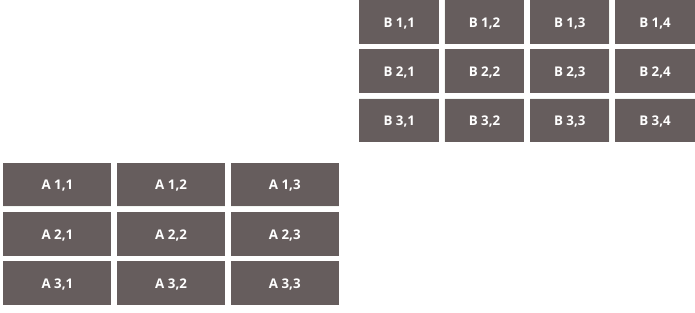
\includegraphics[width=.8\textwidth, keepaspectratio]{assets/matmul_1.png}
%             }
%             \only<3> {
%                 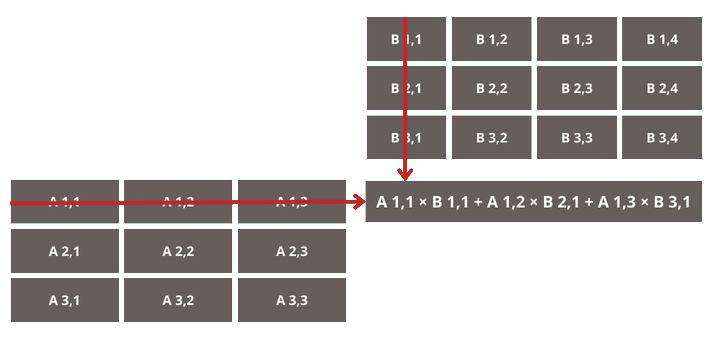
\includegraphics[width=.8\textwidth, keepaspectratio]{assets/matmul_2.png}
%             }
%             \only<4> {
%                 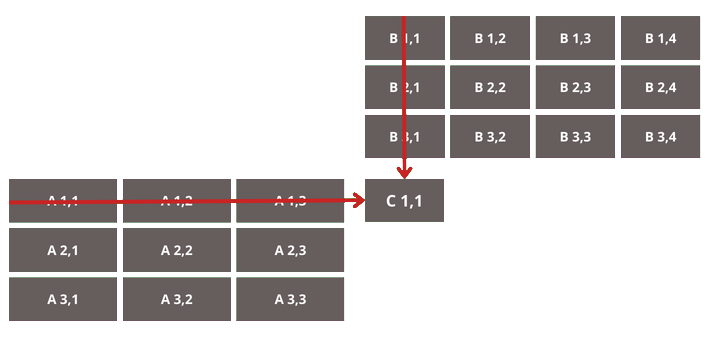
\includegraphics[width=.8\textwidth, keepaspectratio]{assets/matmul_3.png}
%             }
%             \only<5> {
%                 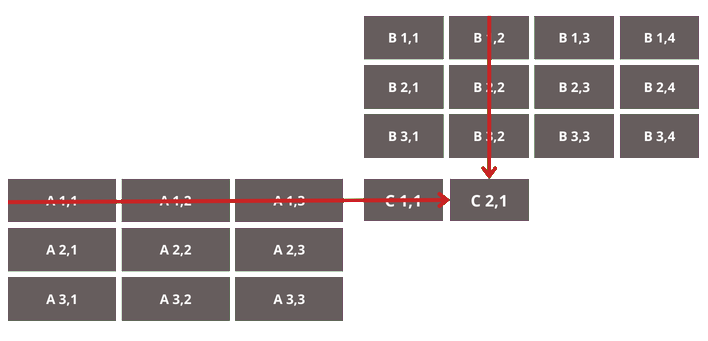
\includegraphics[width=.8\textwidth, keepaspectratio]{assets/matmul_4.png}
%             }
%             \only<6> {
%                 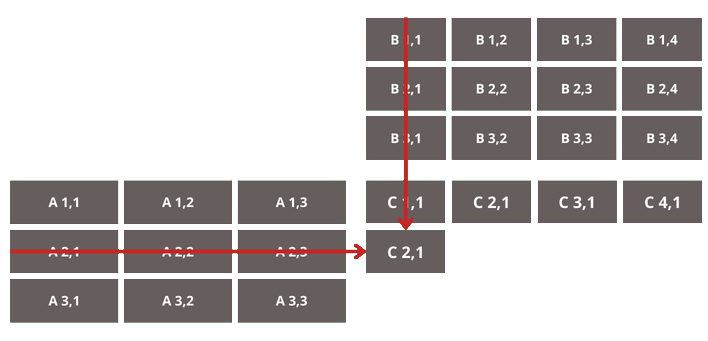
\includegraphics[width=.8\textwidth, keepaspectratio]{assets/matmul_5.png}
%             }
%             \only<7> {
%                 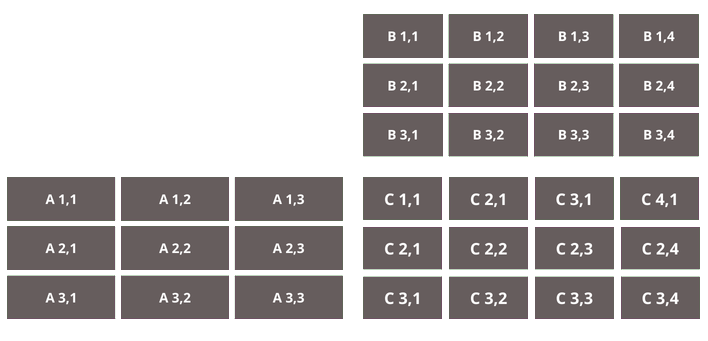
\includegraphics[width=.8\textwidth, keepaspectratio]{assets/matmul_6.png}
%             }
%        \end{itemize}
%     \end{block}
%     \begin{block}<only@8->{Sequential DGEMM \footnote{The D stands for Double Precision Float, the datatype used by the matrix} (GEneral Matrix Multiplication)}
%         \begin{itemize}
%             \item The actual DGEMM operation is $C = \alpha \cdot A \cdot B + \beta \cdot C$. Our work focuses on DGEMM on two non-transposed matrices
%             \item  DGEMM is used in numerous linear algebra kernels such as DTRSM, and DGETRF for example
%             \item Even parallel DGEMM require a sequential kernel at some point
%         \end{itemize}
%         For all those reasons, a GEMM kernel must be as efficient as possible in order not to be the bottleneck for other operations.\\
%     \end{block}
% \end{frame}

% \begin{frame}{First implementations}
%     \begin{block}{Considerations}<only@1-3>
%         \begin{itemize}
%             \item The order of operation  defines the way you will access memory.\\
%             We need to make sure we access memory as contiguously as possible.
%             \item<2-> Use cache as much as possible in order to avoid RAM high latency.\\
%             Using a blocking approach cutting the matrices into smaller matrices that fit in caches.
%             \item<3-> Our goal is to maximize the use of one single CPU core.\\
%             Make use of the instruction sets available on PlaFRIM, AVX2 and FMA.
%         \end{itemize}
%     \end{block}
%     \begin{block}{Implementations}<only@4>
%     \begin{itemize}
%         \item Scalar version\\
%         \item Block version\\
%         \item AVX2 version\\
%         \item Combining AVX2 and Blocking\\
%     \end{itemize}
%     \end{block}
%     \begin{block}{Results for square matrices ($M=N=K$)}<only@5>
%         \vspace{12pt}
%         \only<5>{
%             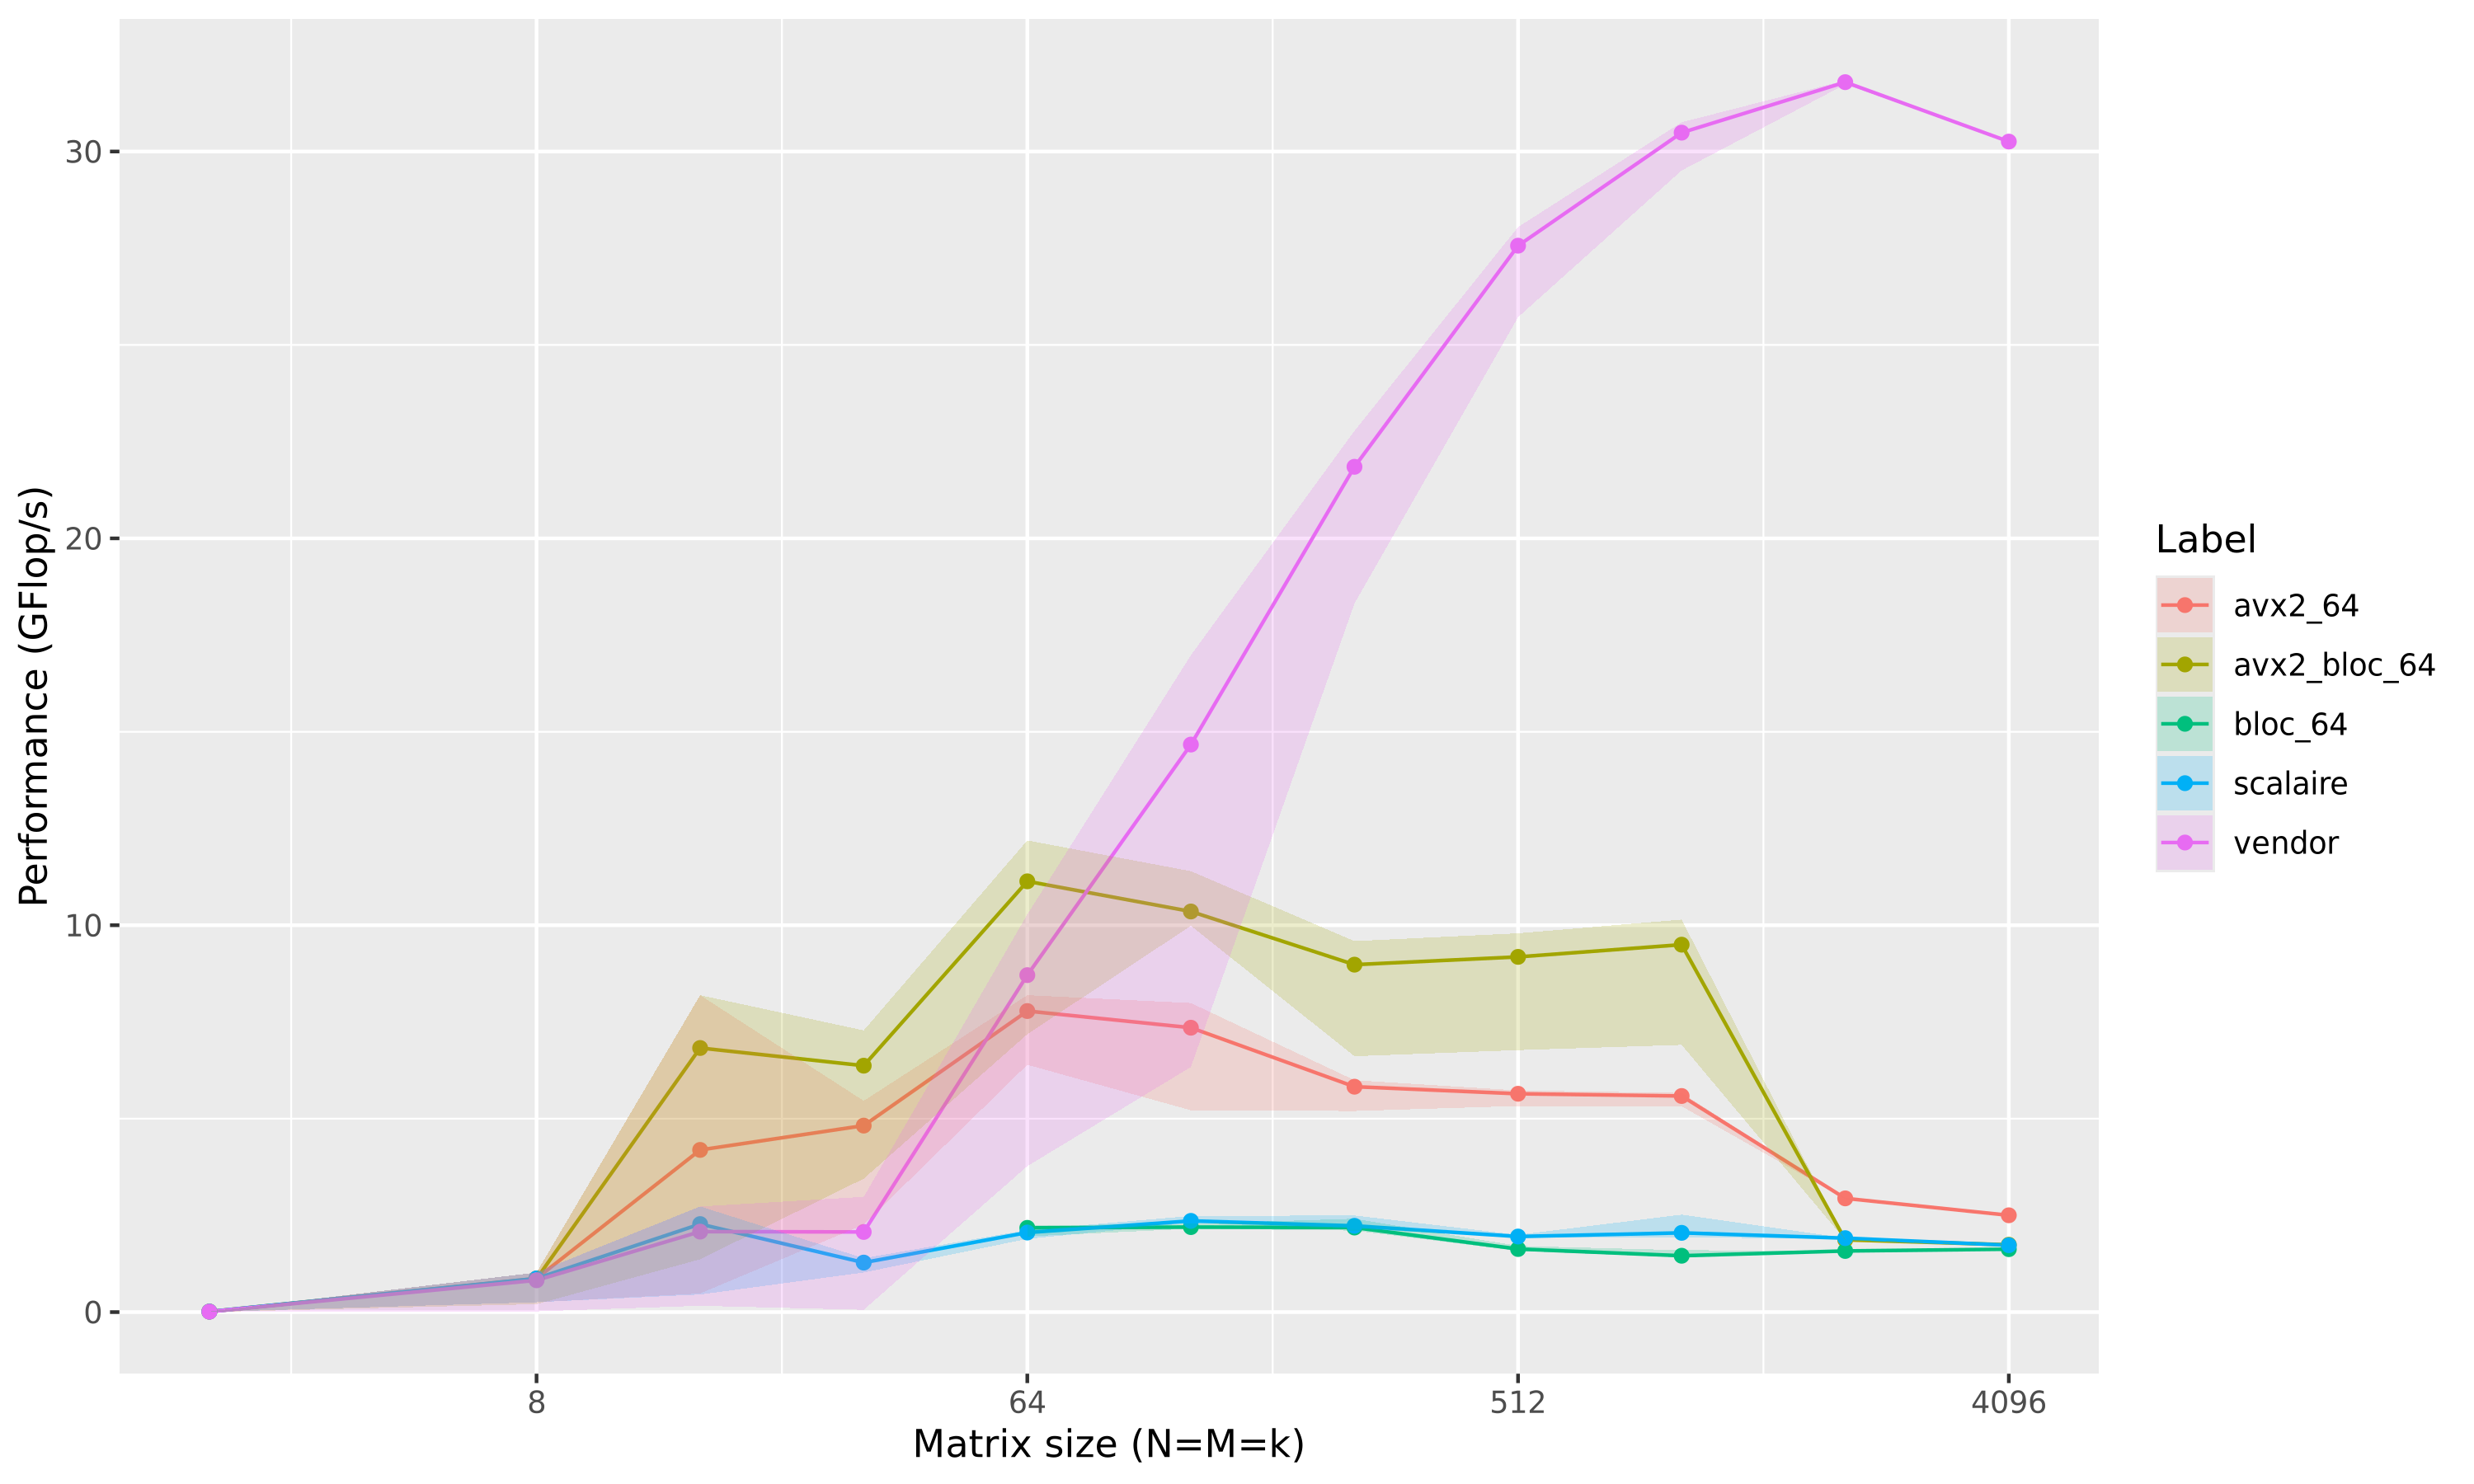
\includegraphics[width=1\textwidth, keepaspectratio]{assets/all_naive.png}
%         }
%     \end{block}
%     \begin{block}{Observations}<only@6>
%         \begin{itemize}
%             \item Peek of performances is reach very early, performances ends up collapsing when $M \times N \sim 1024 \times 1024$
%             \item Blocking algorithm seem to make much more of a difference when combined with vectorization
%             \item As we can see, we are heavily bounded by the RAM accesses, meaning we don't use caches enough
%                 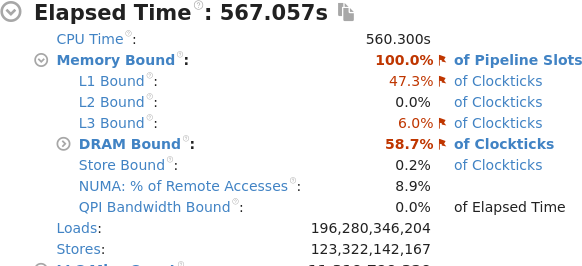
\includegraphics[width=.8\textwidth]{assets/naive_vtune_mem.png}
%         \end{itemize}
%     \end{block}
%     \begin{block}{Conclusions}<only@7>
%         \begin{itemize}
%             \item There is quite a lot of space for improvements
%             \item We need to focus on cache utilization and arithmetic intensity
%             \item Lot of research exists on that topic, so let's not reinvent the wheel
%         \end{itemize}
%     \end{block}
% \end{frame}
\begin{frame}{The need for an efficient DGEMM}
    \begin{block}{Sequential DGEMM}
        \begin{itemize}
            \item  DGEMM is used in numerous linear algebra kernels such as DTRSM, and DGETRF for example
            \item Even parallel DGEMM require a sequential kernel
        \end{itemize}
    In order to avoid getting bottleneck by our sequential DGEMM, it needs to be as efficient as possible.
    \end{block}
\end{frame}
\begin{frame}{Research on efficient DGEMM}
    Most of recent work concerns parallel DGEMM or mixed-precision GEMM.\\
    Three articles seemed interesting:
    \begin{itemize}
        \item Improving the Performance of DGEMM with MoA and Cache-Blocking, Thomas et al., 2021
        \item Anatomy of High-Performance Matrix Multiplication, Goto and Van De Geijn, 2008
        \item Analytical Modeling Is Enough for High-Performance BLIS, Meng Low et al.
    \end{itemize}
    We went with Goto as:
    \begin{itemize}
        \item The underlying algorithm is fairly simple to understand
        \item It has been widely used inside of GotoBLAS
    \end{itemize}
\end{frame}
\begin{frame}{GOTO}
    \only<1>{
        \begin{block}{High Level Overview}
            4 operations:
            \begin{itemize}
                \item GEMM (Matrix x Matrix)
                \item GEPP (Panel x Panel)
                \item GEBP (Block x Panel)
                \item Microkernel
            \end{itemize}
        \end{block}
    }
    \only<2>{
        \begin{block}{GEMM}
            \centering
            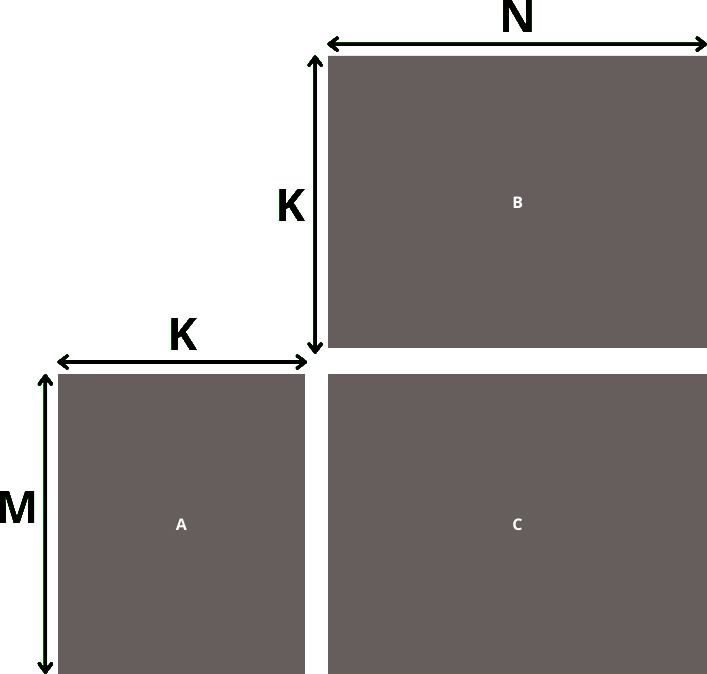
\includegraphics[height=.8\textheight, keepaspectratio]{assets/goto_1.png}
        \end{block}
    }
    \only<3>{
        \begin{block}{GEPP}
            \centering
            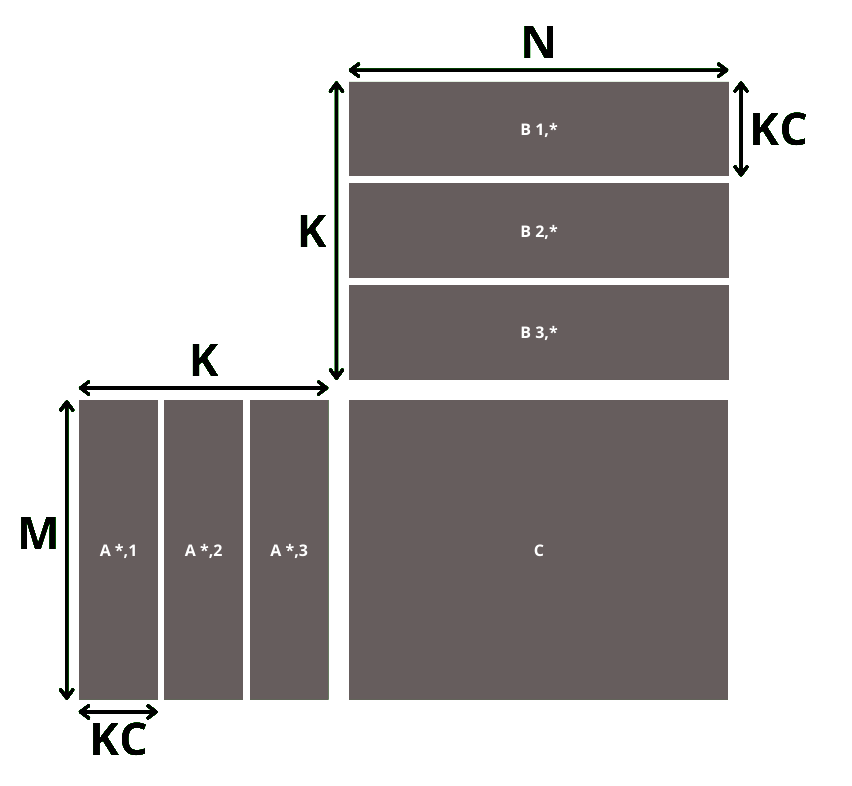
\includegraphics[height=.8\textheight, keepaspectratio]{assets/goto_2.png}
        \end{block}
    }
    \only<4>{
        \begin{block}{GEBP}
            \centering
            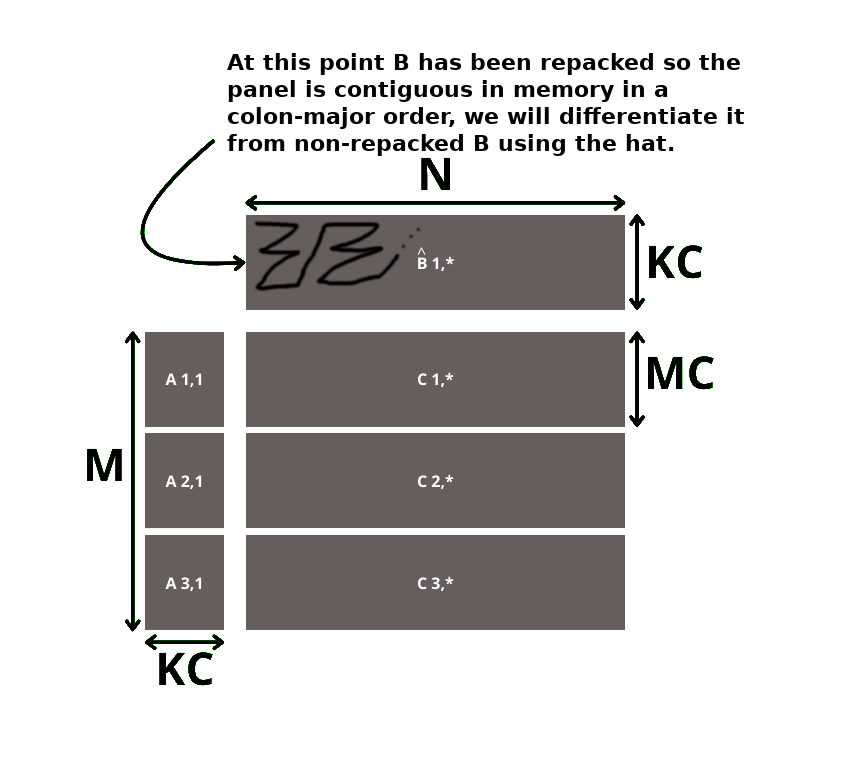
\includegraphics[height=.8\textheight, keepaspectratio]{assets/goto_3.png}
        \end{block}
    }
    \only<5>{
        \begin{block}{GEBP (bis)}
            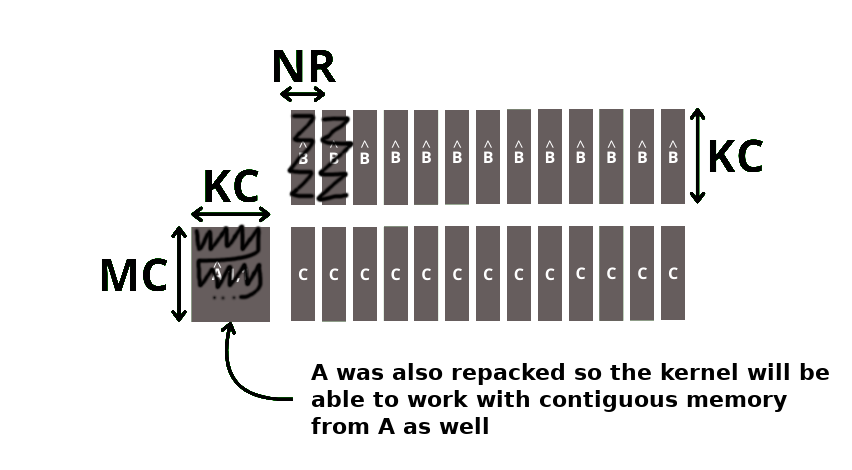
\includegraphics[width=1\textwidth, keepaspectratio]{assets/goto_4.png}
        \end{block}
    }
    \only<6>{
        \begin{block}{Microkernel}
            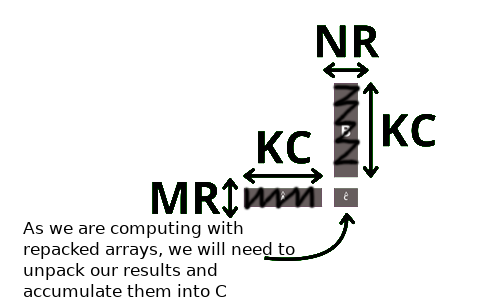
\includegraphics[height=.8\textheight, keepaspectratio]{assets/goto_5.png}
        \end{block}
    }
    \only<7>{
        \begin{block}{Microkernel Implementation}
            \vspace*{1pt}
\begin{itemize}
            \item 10 out of the 16 available vectorial registers
            \item Oblivious to the true matrix size
            \item Loop unrolling to avoid conditional jumps
            \item Aligned load/store thanks to repacking
            \item MR = 4, NR = 8
        \end{itemize}

        \end{block}
        \begin{block}{Testbed}
            \begin{itemize}
                \item Intel Xeon CPU E5-2680 v3, limited at 2.50GHz
                \item 24 threads, AVX2 + two FMA units, getting up to 40Gflop/s in double precision
                \item 32Kb L1 cache, 256Kb L2 cache, ~15Mb L3 cache
            \end{itemize}
        \end{block}
            }
    \only<8-9>{
        \begin{block}{Results for square matrices ($M = N = K$)}<only@8>
            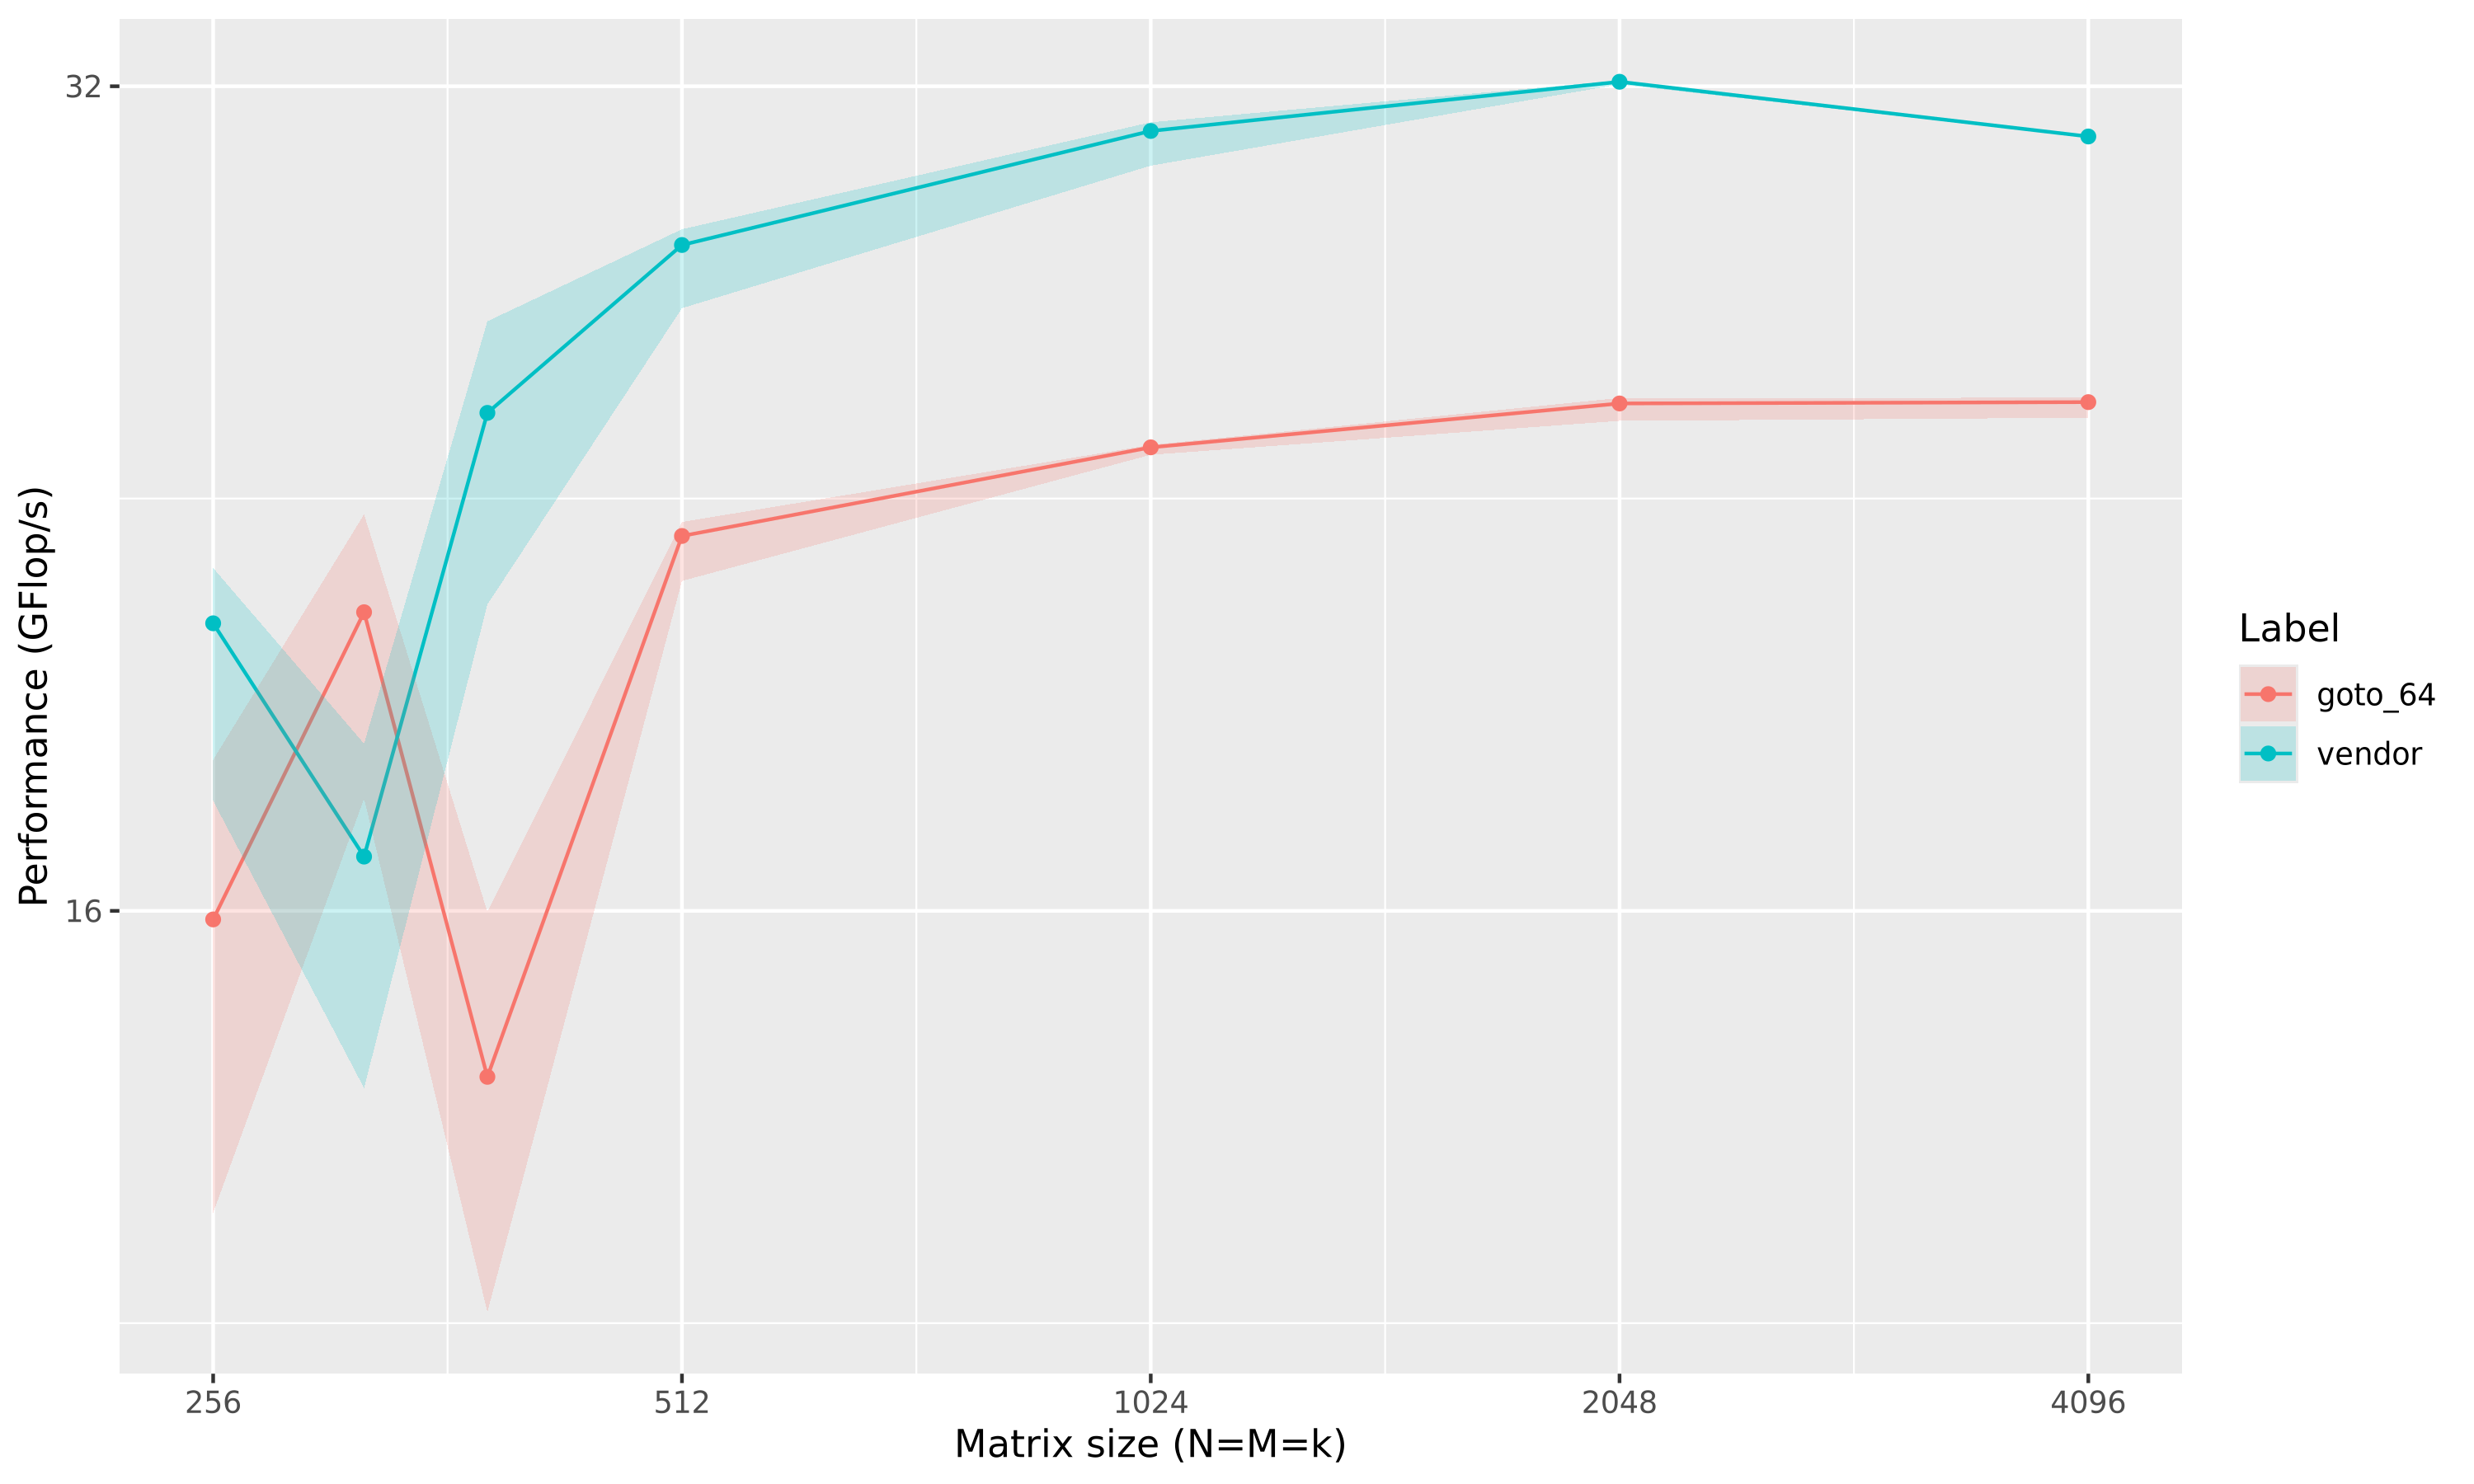
\includegraphics[height=.8\textheight, keepaspectratio]{assets/goto_vs_vendor.png}
        \end{block}
        \begin{block}{Impact of Goto on memory accesses}<only@9>
            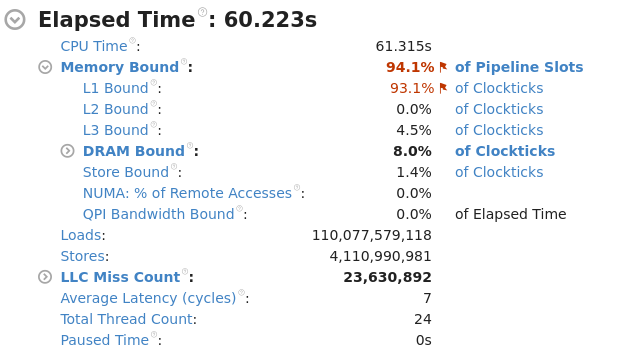
\includegraphics[height=.8\textheight, keepaspectratio]{assets/goto_vtune_mem.png}
        \end{block}
    }
    \only<10>{
        \begin{block}{Sequential DGEMM implementation}
        \begin{itemize}
            \item We managed to get from less than 10 GFlop/s peeks up to 25GFlop/s, reaching up to 75\% of OpenBLAS speed
            \item We are now bounded by L1 cache accesses. There are still place for ameliorations, probably  better cache management and handwritten assembly
            \item We have a solid sequential CPU DGEMM to work with
        \end{itemize}
        \end{block}
    }
\end{frame}
